
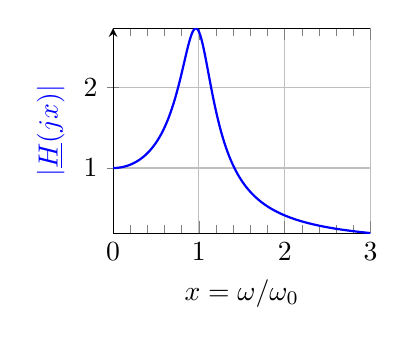
\begin{tikzpicture}[declare function={ 
																			qualite=2.5;
																			om=1;
																			H(\x)=sqrt((1+\x*\x/qualite/qualite)/(1+\x*\x*\x*\x-2*\x*\x+(\x*\x/qualite/qualite)));
																			maximum=3; % échelle linéaire
																			maxlog=100; %échelle log
																			}]

\begin{axis}[width=.4\columnwidth,
                        xmin=0,
                        xmax=maximum,
                        axis y line=left,
                        ylabel= \textcolor{blue}{$|\underline{H}(jx)|$},
                        xlabel={ $x=\omega/\omega_0$},
                       grid = major,
	                   xtick={0,1,..., maximum},
                       minor x tick num = 4,
                       ]    
        
\addplot+[thick, blue, mark=none, samples=150, domain=0:maximum, smooth] {H(x))};
\end{axis}
\end{tikzpicture}
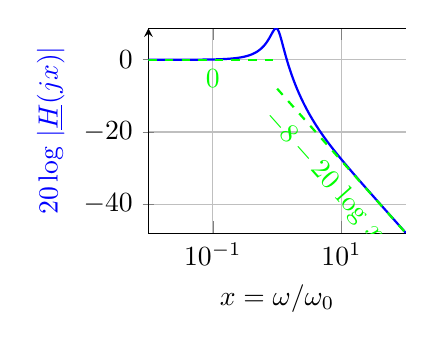
\begin{tikzpicture}[declare function={ 
																			qualite=2.5;
																			om=1;
																			H(\x)=sqrt((1+\x*\x/qualite/qualite)/(1+\x*\x*\x*\x-2*\x*\x+(\x*\x/qualite/qualite)));
																			maximum=3*om; % échelle linéaire
																			maxlog=100; %échelle log
																			GdB(\x)=20*log10(\x);
																			}]

 \begin{semilogxaxis}[width=.4\columnwidth,
										       xmin={1/maxlog},
										       xmax={1*maxlog},
										       axis y line=left,
										       ylabel= \textcolor{blue}{$20\log\,|\underline{H}(jx)|$},
										       xlabel={ $x=\omega/\omega_0$},
										       grid = major,
										       minor x tick num = 4,
										       ]    
        \addplot+[thick, mark=none, blue, samples=150, domain=om/maxlog:om*maxlog, smooth] {GdB(H(x)))};
        \addplot+[thick, dashed, green, mark=none, samples=10, domain=om/maxlog:1, smooth] {0} node [midway, sloped, below] {$0$}; 
       \addplot+[thick, dashed,  green, mark=none, samples=10, domain=1:maxlog, smooth] {-8-20*log10(x)} node [midway, sloped, below] {$-8-20\,\log\,x$}; ;
\end{semilogxaxis}
\end{tikzpicture}